%! Author = evert
%! Date = 21-7-2024
\section{Research methodology}
The research methodology consists of creating an Agent Based Model in NetLogo, deciding the behaviour rules of the agents and program them in the model, conduct
experiments by running simulations in which different variables are set.

The model details, and result will be presented in a paper.

The model based approach is a way to eliminate all variables not direct related to the problem and keep only the essence of the situation.
Also, a real world experiment is not possible, at least not for a single researcher.

The environment where multiple agents act is called a multi-agent system end the problem is called a multi-agent planning problem (from~\cite{russell2016artificial}).
The research problem is actually a comparison between a system where there is one decision maker (the company assigns delivery jobs) and a system where each deliverer decide for its self (multiple decision makers).
This research will not be of a thoroughly theoretical nature though, its more of an exploratory/explanatory nature, see what happens under some conditions and explain the correlation.

The nature of a NetLogo model is that in each step, a time unit, all actors do something (or do nothing) but the order in which the actors do something is random.
There is an interleaved execution of events, no race conditions take place, this solves the problem of who gets a delivery job in case of several free deliverers.

An effort will be made to search for existing NetLogo models that can be reused.

First example: a grid with roads is used in the Taxi Cab model~\cite{dongpingtaxicabs2019} as shown in figure~\ref{fig:taxi cab}
\begin{figure}
    \centering
    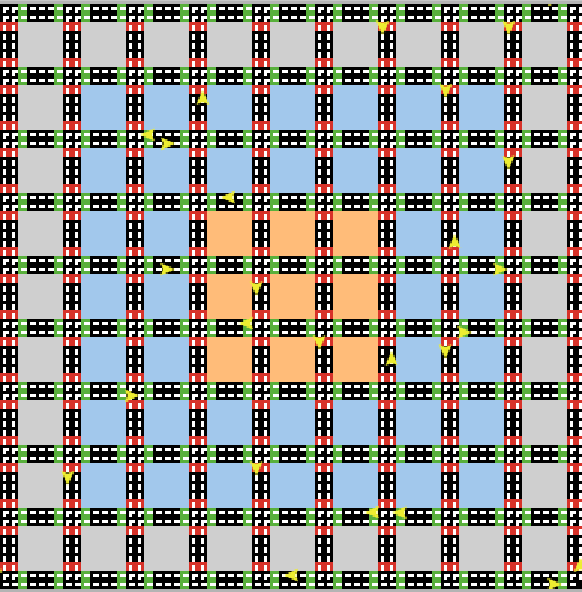
\includegraphics[width=6cm]{sections/pics/Taxi Cabs}
    \caption{Taxi Cab Model}
    \label{fig:taxi cab}
\end{figure}

Second example: the simulation is used in ~\cite{ismail2024software}.
In this study some rules, goals and tasks are listed, shown in figure~\ref{fig:tasktable} , that can be adapted and used in our model.
The NetLogo ui of this model is shown in figure~\ref{fig:a-ride}.
\begin{figure}
    \centering
    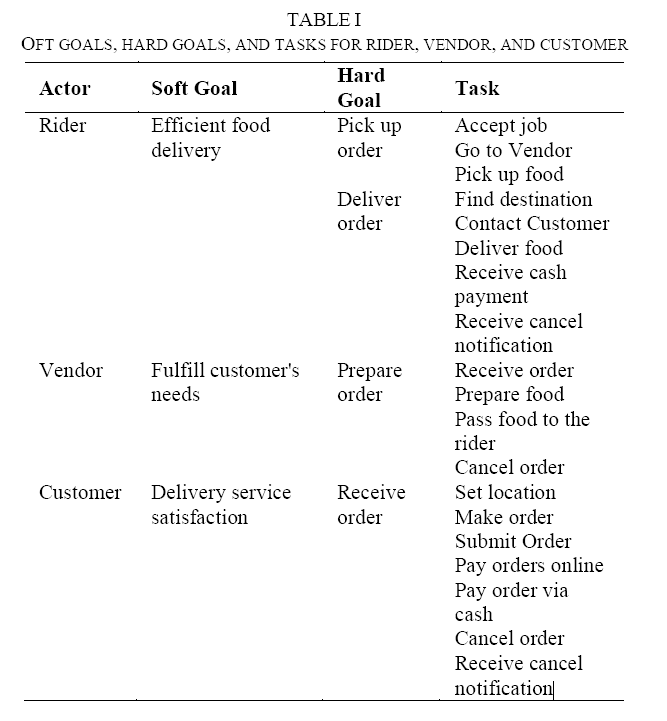
\includegraphics[width=8cm]{sections/pics/TaskTabel}
    \caption{Food Delivery}
    \label{fig:tasktable}
\end{figure}

\begin{figure*}
    \centering
    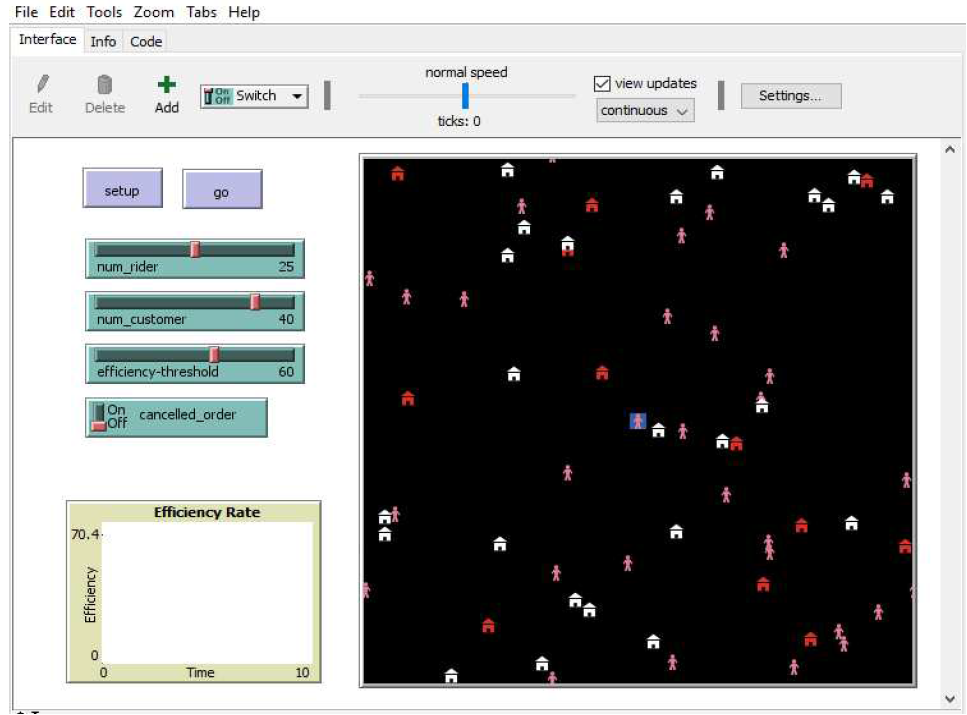
\includegraphics[width=\linewidth]{sections/pics/a-ride}
    \caption{NetLogo a-ride simulation}
    \label{fig:a-ride}
\end{figure*}
